\documentclass{article}

\usepackage{amsmath}
\usepackage{amsfonts}
\usepackage{amssymb}
\usepackage{textcomp, gensymb}
\usepackage[dvipsnames]{xcolor}
\usepackage[margin=0.5in]{geometry}
\usepackage[hidelinks]{hyperref}

\usepackage{environ}
\NewEnviron{centerframebox}{\begin{center}\fbox{\parbox{0.92\textwidth}{\BODY}}\end{center}}

\usepackage{tasks}
\usepackage{wrapfig}
\usepackage{tikz}
\usetikzlibrary{patterns}

\pgfdeclarepatternformonly{south east lines}{\pgfqpoint{-0pt}{-0pt}}{\pgfqpoint{3pt}{3pt}}{\pgfqpoint{3pt}{3pt}}{
  \pgfsetlinewidth{0.4pt}
  \pgfpathmoveto{\pgfqpoint{0pt}{3pt}}
  \pgfpathlineto{\pgfqpoint{3pt}{0pt}}
  \pgfpathmoveto{\pgfqpoint{.2pt}{-.2pt}}
  \pgfpathlineto{\pgfqpoint{-.2pt}{.2pt}}
  \pgfpathmoveto{\pgfqpoint{3.2pt}{2.8pt}}
  \pgfpathlineto{\pgfqpoint{2.8pt}{3.2pt}}
  \pgfusepath{stroke}}

\let\oldphi\phi
\let\phi\varphi

\newcommand{\N}{\mathbb{N}}
\newcommand{\R}{\mathbb{R}}
\newcommand{\C}{\mathbb{C}}

\title{Quantum Algorithms \\ Exercise 1}
\author{
  \AA{AAAAAAAAAA AAAAAAA}{6} \\ \href{mailto:\AA{AAAAAAAAAAAAAAAAAAAA}{7}}{\AA{AAAAAAAAAAAAAAAAAAAA}{7}} \and
  Chuong Dinh Le \\ \href{mailto:s56dle@uni-bonn.de}{s56dle@uni-bonn.de} \and
  Paul Berners \\ \href{mailto:s6plbern@uni-bonn.de}{s6plbern@uni-bonn.de} \and
  Fynn Osterfeld \\ \href{mailto:s6fyoste@uni-bonn.de}{s6fyoste@uni-bonn.de}
}

\begin{document}
  \maketitle

  \setcounter{section}{1}
  \subsection{Complex Numbers}
  \subsubsection*{(A) Euler's formula}
  \begin{centerframebox}
    Calculate the complex number given by $re^{i\phi}$ for $r = 1$ and:
    \begin{tasks}[style=itemize](4)
      \task $\phi = 0$
      \task $\phi = \frac{\pi}{2}$
      \task $\phi = \pi$
      \task $\phi = \frac{3\pi}{2}$
    \end{tasks}
  \end{centerframebox}
  \begin{wrapfigure}{r}{4cm}
    \vspace{-.5cm}
    \centering
    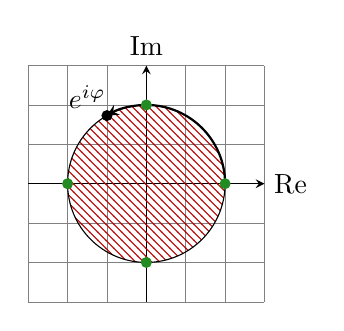
\begin{tikzpicture}[x=.5cm,y=.5cm]
      \draw[step=1, gray, very thin] (-3,-3) grid (3,3);
      \draw[-stealth] (-3,0)--(3,0) node[right]{Re}; % x axis
      \draw[-stealth] (0,-3)--(0,3) node[above]{Im}; % y axis

      \draw[pattern=south east lines, pattern color=BrickRed] (0,0) circle[radius=2];

      \draw[->,>=stealth,thick] (2,0) arc[radius=2, start angle=0, end angle=120];
      \node (a) at (-1,2.2) {$\hspace{-.5cm}e^{i\phi}$};
      \fill (-1,1.73) circle[radius=2pt];

      \fill[fill=ForestGreen] (0,2) circle[radius=2pt];
      \fill[fill=ForestGreen] (2,0) circle[radius=2pt];
      \fill[fill=ForestGreen] (0,-2) circle[radius=2pt];
      \fill[fill=ForestGreen] (-2,0) circle[radius=2pt];
    \end{tikzpicture}
  \end{wrapfigure}

  The expression we need to calculate is actually Euler's Formula.
  It allows us to write any complex number in terms of its magnitude and its angle with the real axis.
  The values of $\phi$ we were given correspond directly to multiples of $90\degree = \frac{\pi}{2}$.
  The value of $r$ is $1$ so we don't have to change the magnitude of the resulting complex number,
  and it will just stay on the unit circle.
  From trigonometry we get the formula $e^{i\phi} = \cos \phi + i\sin \phi$,
  but in our particular case the angles are so simple, that we only get values of $\pm 1$ and $0$.

  So for our values of get: \\
  \begin{tabular}{lllllll}
    \textbullet $\quad\phi = 0$ & $\qquad\to\qquad$ & $re^{i\phi} = 1$ & $\qquad\qquad$ &
    \textbullet $\quad\phi = \frac{\pi}{2}$ & $\qquad\to\qquad$ & $re^{i\phi} = i$ \\
    \textbullet $\quad\phi = \pi$ & $\qquad\to\qquad$ & $re^{i\phi} = -1$ & $\qquad\qquad$ &
    \textbullet $\quad\phi = \frac{3\pi}{2}$ & $\qquad\to\qquad$ & $re^{i\phi} = -i$ \\
  \end{tabular}

  \subsubsection*{(B) Wave function}
  \begin{centerframebox}
    A wave function $\psi(x)$ for some state $x_0$ is given by $\psi(x_0) = \frac{1}{2} + \frac{1}{2}i$.
    \begin{itemize}
      \item What is the probability density $p(x_0)$?
      \item Calculate the factor $\gamma$ such that $\gamma\psi(x_0) = -\frac{1}{2}$.
    \end{itemize}
  \end{centerframebox}
  The probability density of a wave function is generally given by its square magnitude.
  Because we know the value of $\psi(x_0)$, we can just square it by hand.
  \begin{align*}
    p(x_0) &= |\psi(x_0)^2| \\
    &= \left|\left(\frac{1}{2} + \frac{1}{2}i\right)^2\right| \\
    &= \left|\left(\frac{1}{2} + \frac{1}{2}i\right) \cdot \left(\frac{1}{2} + \frac{1}{2}i\right)\right| \\
    &= \left|\frac{1}{2}\frac{1}{2} + \frac{1}{2}\frac{1}{2}i + \frac{1}{2}\frac{1}{2}i + \frac{1}{2}\frac{1}{2}i^2\right| \\
    &= \left|\frac{1}{4} + \frac{1}{2}i - \frac{1}{4}\right| \\
    &= \left|\frac{1}{2}i\right| \\
    &= \frac{1}{2} \\
  \end{align*}
  The probability turned out to be $0.5$!

  Now to calculate the factor $\gamma$, we just need to solve the equation $\gamma\psi(x_0) = -\frac{1}{2}$ with some simple algebra.
  We just need to divide both sides by $\psi(x_0)$, because it's just a complex number we know.
  \begin{align*}
    \gamma &= -\frac{1}{2} \cdot \psi(x_0)^{-1} \\
    &= -\frac{1}{2} \cdot \frac{\bar\psi(x_0)}{|\psi(x_0)|^2} \\
    &= -\frac{1}{2} \cdot \frac{\frac{1}{2} - \frac{1}{2}i}{\frac{1}{2}} \\
    &= -\frac{2}{2} \cdot \left(\frac{1}{2} - \frac{1}{2}i\right) \\
    &= -\frac{1}{2} + \frac{1}{2}i \\
  \end{align*}

  So $\gamma = -\frac{1}{2} + \frac{1}{2}i$, and we can even verify it work by multiplying it again.

  \subsection{Schrödinger Equation}
  \subsubsection*{(A) Derivation}
  \begin{centerframebox}
    Derive the time-independent Schrödinger equation from the time-dependant by using the time independent Hamiltonian.

    \begin{tasks}[style=itemize](2)
      \task Time-dependant Schrödinger equation \\
      \begin{center} $\displaystyle i\hbar \frac{\partial \Psi(x,t)}{\partial t}  = \hat{H} \Psi(x,t) $ \end{center}
      \task Time-independent Schrödinger equation \\
      \begin{center} $\displaystyle \hat{H} \psi(x) = E \psi(x) $ \end{center}
    \end{tasks}
  \end{centerframebox}
  First, because we are working in the time-independent case, we can assume that the wave function $\Psi(x,t)$
  can be separated into a space dependant and a time dependant component $\Psi(x,t) = \psi(x) u(t)$.

  Substituting this into the time-dependant Schrödinger equation:
  \begin{align*}
    i\hbar \frac{\partial \psi(x) u(t)}{\partial t} &= \hat{H} \psi(x) u(t) \\
    i\hbar \left( \psi(x)\frac{\partial u(t)}{\partial t} + u(t)\frac{\partial \psi(x)}{\partial t} \right) &= \\
    i\hbar \left( \psi(x)\frac{\partial u(t)}{\partial t} + u(t) \cdot 0 \right) &= \\
    i\hbar \psi(x)\frac{\partial u(t)}{\partial t} &= \hat{H} \psi(x) u(t) \\
    i\hbar \frac{\partial u(t)}{\partial t} &= \hat{H} u(t) \\
  \end{align*}

  If we assume $u(t)$ only contains a complex phase component $u(t) = e^{-\frac{i}{\hbar}Et}$,
  where $E$ is just some scaling constant (for now),
  and substitute it into the differential equation we got from the last line, we get:
  \begin{align*}
    i\hbar \frac{\partial u(t)}{\partial t} &= \hat{H} u(t) \\
    i\hbar \cdot \left( {-\frac{i}{\hbar}E} \right) u(t) &= \hat{H} u(t) \\
    E u(t) &= \hat{H} u(t)
  \end{align*}

  We can conclude that $E$ must be the energy eigenvalue and $u(t) = e^{-\frac{i}{\hbar}Et}$.
  Now we substitute this into the original equation we had, before we removed $\psi(x)$.
  \begin{align*}
    i\hbar \psi(x)\frac{\partial u(t)}{\partial t} &= \hat{H} \psi(x) u(t) \\
    \psi(x) E u(t) &= \hat{H} \psi(x) u(t) \\
    E\psi(x) &= \hat{H} \psi(x) \\
  \end{align*}
  This is the time-independent Schrödinger equation, and we're done.
  $\blacksquare$

  \subsubsection*{(B) Linearity}
  \begin{centerframebox}
    Let be $\Psi,\, \Phi$  solutions of the Schrödinger equation.
    Show that the Schrödinger equation is linear, i.e. $\alpha\Psi + \beta\Phi$ are also solutions for $\alpha,\, \beta \in \C$.
  \end{centerframebox}

  Since the partial derivation operation $\partial$ is linear, this becomes very clear:
  \begin{align*}
      i\hbar \frac{\partial\left(\alpha\Psi + \beta\Phi\right)(x, t)}{\partial t} &= i\hbar \frac{\alpha\partial\Psi(x, t)+\beta\partial\Phi(x, t)}{\partial t}\\
      &= i\hbar \frac{\alpha\partial\Psi(x, t)}{\partial t} + i\hbar \frac{\beta\partial\Phi(x, t)}{\partial t}\\
      &= \alpha \left(i\hbar \frac{\partial\Psi(x, t)}{\partial t}\right) + \beta \left(i\hbar \frac{\partial\Phi(x, t)}{\partial t}\right)\\
      &= \alpha \hat{H}\Psi(x, t) + \beta \hat{H}\Phi(x, t)\\
      &= \hat{H}(\alpha\Psi + \beta\Phi)(x, t)
  \end{align*}

  \subsection{The Free Particle}
  \begin{centerframebox}
    The free particle moves with some given kinematic energy without being exposed to any potential
    ($V = 0$). As a consequence, the Hamiltonian is given by

    \[ \hat{H}(x) = \frac{\hat{p}^2}{2m} = -\frac{\hbar^2}{2m}\frac{\partial^2}{\partial x^2} \]

    \begin{itemize}
      \item Show that the following wave function $\Psi$ is a solution to the Schrödinger equation:
      \[ \Psi(x,\, t) = \exp\left(\frac{i}{\hbar} (px-Et)\right) \]
      \item The momentum operator is given by $\hat{p} = -i\hbar\dfrac{\partial}{\partial x}$. Show that $\hat{p}\Psi = p\Psi$.
      \item The energy operator is given by $\hat{E} = i\hbar\dfrac{\partial}{\partial t}$. Show that $\hat{E}\Psi = E\Psi$.
    \end{itemize}
  \end{centerframebox}
  \begin{itemize}
    \item[] We have
        $e^{\frac{i}{\hbar}(px-Et)} = e^{i(\frac{p}{\hbar}x-\frac{E}{\hbar}t)} \Rightarrow E = \frac{\hbar^2k^2}{2m} = \frac{\hbar^2\frac{p}{\hbar}^2}{2m} = \frac{p^2}{2m}$ (1)
    \item[] Substitute $\psi(x)$ to Schroedinger equation:
    \begin{align*}
        &-\frac{\hbar^2}{2m}\frac{\partial^2 \psi(x)}{\partial^2 x} = E\psi(x)\\
        &\Leftrightarrow -\frac{\hbar^2}{2m}(\frac{ip}{\hbar})^2\psi(x) = E\psi(x)\\
        &\Leftrightarrow \frac{p^2}{2m}\psi(x) = E\psi(x) \label{eq}
    \end{align*}
    \item[] By substitute $E$ from (1), the equation holds true. Hence, the given $\psi(x)$ is a solution to the Schroedinger equation.
  \end{itemize}



  So calculate both sides of the Schrödinger equation:
  \begin{align*}
      i\hbar\frac{\partial\Psi(x, t)}{\partial t} &= i\hbar\left(-\frac{i}{\hbar}E\exp{\left(\frac{i}{\hbar}(px-Et)\right)}\right)\\
      &= E\exp{\left(\frac{i}{\hbar}(px-Et)\right)}\\
      &= E\Psi(x, t)
  \end{align*}
  \begin{align*}
      \hat{H}\Psi(x, t) &= \frac{\hbar^2}{2m}\frac{\partial}{\partial x^2}\exp{\left(\frac{i}{\hbar}(px-Et)\right)}\\
      &= \frac{\hbar^2}{2m}\frac{i^2}{\hbar^2}p^2\exp{\left(\frac{i}{\hbar}(px-Et)\right)}\\
      &= -\frac{p^2}{2m}\exp{\left(\frac{i}{\hbar}(px-Et)\right)}\\
      &= -\frac{p^2}{2m}\Psi(x, t)
  \end{align*}
  Then $E = -\frac{p^2}{2m}$ is equivalent to $\Psi$ being a solution of the Schrödinger equation.\\\\
  To show $\hat{p}\Psi = p\Psi$ just calculate $\hat{p}\Psi$:
  \begin{align*}
      \hat{p}\Psi(x, t) &= -i\hbar\frac{\partial}{\partial x}\exp{\left(\frac{i}{\hbar}(px-Et)\right)}\\
      &= -i\hbar\frac{i}{\hbar}p\exp{\left(\frac{i}{\hbar}(px-Et)\right)}\\
      &= p\exp{\left(\frac{i}{\hbar}(px-Et)\right)}\\
      &= p\Psi(x, t)
  \end{align*}
  To show $\hat{E}\Psi = E\Psi$ just calculate $\hat{E}\Psi$:
  \begin{align*}
      \hat{E}\Psi(x, t) &= i\hbar\frac{\partial}{\partial t}\exp{\left(\frac{i}{\hbar}(px-Et)\right)}\\
      &= i\hbar\frac{i}{\hbar}(-E)\exp{\left(\frac{i}{\hbar}(px-Et)\right)}\\
      &= E\exp{\left(\frac{i}{\hbar}(px-Et)\right)}\\
      &= E\Psi(x, t)
  \end{align*}
\end{document}
